\documentclass[12pt, letterpaper]{article}
\usepackage[utf8]{inputenc}
\usepackage{graphicx}
\usepackage{hyperref}
\usepackage{fancyvrb}
\usepackage{array}
\usepackage{biblatex}
\usepackage{float}
\usepackage{subcaption}

\bibliography{rapport}

\title{Détection du Cancer de la peau à partir du Convolutional Neural Network}
\author{Komlan Jean-Marie DANTODJI
\\
    \multicolumn{1}{
        p{.7\textwidth}}{\centering\emph{Université Paris Vincennes St-Denis\\
  M1 Big Data\\}
  }
}
\date{Dimanche, 24 janvier 2021}
\begin{document}


\begin{titlepage}
    \maketitle
\end{titlepage}

\tableofcontents

\newpage
\section{Introduction}
\par Le cancer de la peau est une maladie causée par des cellules cancéreuses qui attaquent la peau et qui se développent s’ils n’ont pas été détectés et guéries à temps. Plus le temps s’écoule plus les cellules se multiplient et plus les complications sont difficile à contenir. Aujourd’hui l’évolution de la technologie de l’intelligence artificielle permet de prendre de l’avance sur les premiers signes. Ceci pour détecter plus rapidement les cellules responsables du cancer de la peau. \\
\section{Problématique}
\par L’objectif ici est dans un premier temps découvrir quelques méthodes existantes dans la détection de cellules cancéreuses. Ensuite nous partiront d’une image de la peau d’un patient, faire des prétraitements spécifiques dans le but de faciliter un bon apprentissage en localisant les zones d’intérêts. Et enfin nous détailleront le model d’apprentissage dans la résolution de notre problème avec du CNN. \\
\section{Etat de l'art}
\par Avant, les dermatologues avaient l’habitude d’analyser la peau des patients à la recherche de cellules cancéreuses. Cette méthode atteint ses limites du moment où on est en face d'un nombre très important d’image de la peau à analyser. Pour les automatiser certains ont mis en place des procédés notamment : \\

\begin{itemize}
		\item Robert Amelard et al:\\
		Ils ont suggérés la correction de l’illumination des images de la peau et une plateforme d’extraction de caractéristiques.
		\item A. Goshtasbya D. Rosemanb S. Binesb C. Yuc A. Dhawand A. Huntleye L. Xua:\\
		Ils ont proposés un réseau de neurone avec le Back-propagation neural network (BNN) et l’Auto-associative neural network.
		\item Ramteke et al. : \\
		Propose une methode dependent de la méthode ABCD dans la reconnaissance de l’évolution de cellules malicieux.
		\item Sibi Salim RB Aswin, J Abdul Jaleel. 2013: \\
		Implémentation du classificateur ANN en MATLAB pour la détection de cellules cancéreux.
\end{itemize}

\section{Skin Cancer Detection Using Image Proceessing}
\subsection{Présentation des auteurs}
\par L’article  "Skin Cancer Detection Using Image Proceessing"  publié dans le journal International Research Journal of Engineering and Technology (IRJET) réalisé par les auteurs :
\begin{itemize}
		\item Uzma Bano Ansari M.E. Student, Department of Computer,TSEC,Mumbai
		\item Tanuja Sarode 2 Associate Professor, Department of Computer, TSEC, Mumbai
\end{itemize}
L’article présente les différentes étapes de prétraitement de l’image de la peau.
\subsection{Les étapes de prétraitement}
\begin{itemize}
		\item Image d'entrée:\\
		Cette image d’entrée est une photo prise par le dermatoscope, cette dernière est un appareil efficasse de prise photo de la peau pour avoir une image de qualité. 
		\begin{figure}[H]
    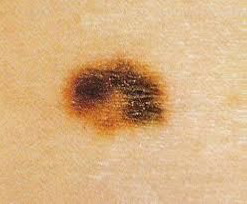
\includegraphics[width=5cm,height=4cm]{images/input_1.png}
    \caption{[1] Input image, page 2879}
    \label{fig:L1}
\end{figure}
		\item Conversion en niveau de gris :\\
Dans le but de réduire le temps d’apprentissage, il serait judicieux de transformer l’image en niveau de gris afin de ne considérer que l’intensité des pixels.
Sa valeur est calculée par la formule suivante :
$$Grayscale intensity = 0.299 R + 0.587 G + 0.114 B$$
		\begin{figure}[H]
    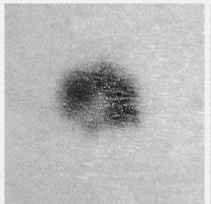
\includegraphics[width=5cm,height=4cm]{images/input_2.png}
    \caption{[1] Gray Scale Image, page 2879}
    \label{fig:L1}
\end{figure}
		\item Réduction de bruits:\\
L’objectif est d’enlever le maximum de bruits indésirables de l’image. Le problème est de savoir quelle caractéristique est réelle ou causé par le bruit. De ce fait la meilleure méthode est de passer l’image sous le filtre médian.
		\begin{figure}[H]
    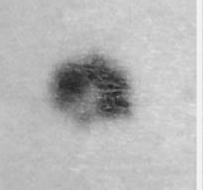
\includegraphics[width=5cm,height=4cm]{images/input_3.png}
    \caption{[1] Image Without Noise, page 2879}
    \label{fig:L1}
\end{figure}
		\item Amélioration de l’image :\\
Ici le but est d’accroitre la visibilité des caractéristiques importantes.
		\begin{figure}[H]
    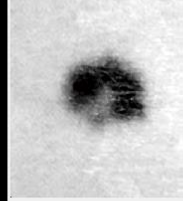
\includegraphics[width=5cm,height=4cm]{images/input_4.png}
    \caption{[1] Enhanced image, page 2879}
    \label{fig:L1}
\end{figure}
		\item Segmentation :\\
 On construit l’histogramme de l’image en niveau de gris pour séparer l’arrière-plan de l’avant-plan avec la méthode du maximum, ce qui donne une image binaire composé que de valeurs 0 et 255. 
		\begin{figure}[H]
    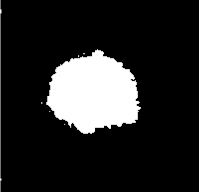
\includegraphics[width=5cm,height=4cm]{images/input_5.png}
    \caption{[1] Segmented Image, page 2880}
    \label{fig:L1}
\end{figure}
\end{itemize}
\section{Base de donnée}

\par Les images d’apprentissage sont des images de la peau des patients prise avec une grande résolution. Pour les tests dans cet article, 23907 images sont collectées de l’archive ISIC. Les images contenant des cellules cancéreuses sont labelisées malsain et sain pour les images non cancéreuses. 

\section{Skin Cancer Detection Using Convolutional Neuronal Network} 

\subsection{Présentation des auteurs}
\par L’article: "Skin Cancer Detection Using Convolutional Neuronal Network" publié dans la revue Researchgate réalisé par quatre auteurs dont:
\begin{itemize}
		\item Mahamudul Hasan de l’Université de Dhaka
		\item Ahmed Wasif Reza de East West University au Bangladesh
\end{itemize}
L’article présente le model du CNN dans la reconnaissance de cellules cancéreuses dans une image.
\subsection{Step 1: Prétraitement}
\par Toutes les images de la base de données sont redimensionnées à la même taille et au minimum de taille possible dans le but de diminuer le temps de traitement. Le même processus est exécuté sur l’image d’entrée. Ensuite toutes ces images sont passées aux traitements détaillés dans la première partie.
\subsection{Step 2: Sauvegarde des images}
\par Sauvegarde des images
Les images prétraitées sont sauvegardées et labélisées afin de les identifier
\subsection{Step 3: Envoie des données d'image au model CNN}
\par A ce stade, à partir de l’image obtenue lors des étapes précédents on passe au calcule de la convolution.\\
Supposons une image de taille 6x6 obtenue, on calcule sa convolution en la passant dans un filtre 3x3. La convolution est calculée par la formule suivante :
$$ \sum_{i=0}^{m-1}\sum_{i=0}^{n-1} X_{(m-i)(n-j)}Y_{(i+1)(j+1)}$$
On calcule la convolution 
\begin{figure}[H]
    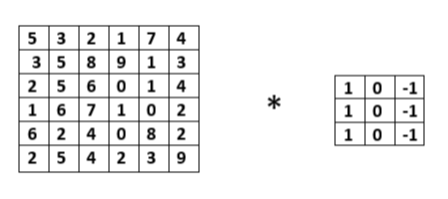
\includegraphics[width=\linewidth]{images/convolution.png}
    \caption{[2] Gray-scale Image 6x6 and the 3x3 filter, page 256}
    \label{fig:L1}
\end{figure}
On obtient la matrice 4x4 de l’image par le filtre:
\begin{figure}[H]
    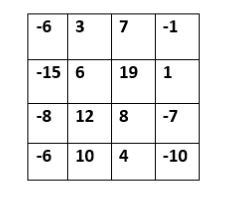
\includegraphics[width=7cm,height=6cm]{images/pooling.png}
    \caption{[2] 4x4 image after applying 3x3 filter to the gray-scale image, page 257}
    \label{fig:L1}
\end{figure}
Pour extraire plus de caractéristiques complexe on peut appliquer le max pooling qui consiste à déterminer le maximum pour chaque block 2x2 de la matrice convoluée.
\begin{figure}[H]
    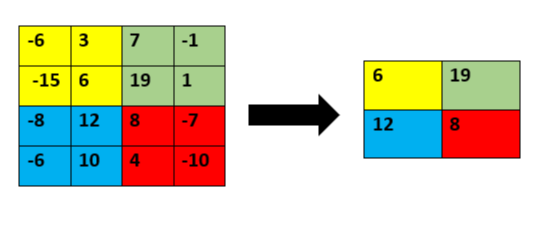
\includegraphics[width=\linewidth]{images/maxpooling.png}
    \caption{[2] Result after applying max pooling, page 257}
    \label{fig:L1}
\end{figure}
\subsection{Step 4: Entrainement}
\par A ce point on entraine le model 200 fois.
\subsection{Step 5: Sauvegarde du model }
\par Après avoir sauvegardé le model on peut alors passer au test de reconnaissance.
\subsection{Step 6: Prédiction}
\par Les images sont envoyés au model pour prédiction et évaluation de l'efficacité du model.
$$ Recall = \frac{TruePositive}{Positive }$$
$$ Specificity = \frac{TrueNegative}{Negative}$$
$$ Precision = \frac{TruePositive}{TruePositive + FalsePositive}$$
$$ Score = \frac{2*Precision*Recall}{Precision+Recall}$$


\section{Discussion} 
\begin{figure}[H]
    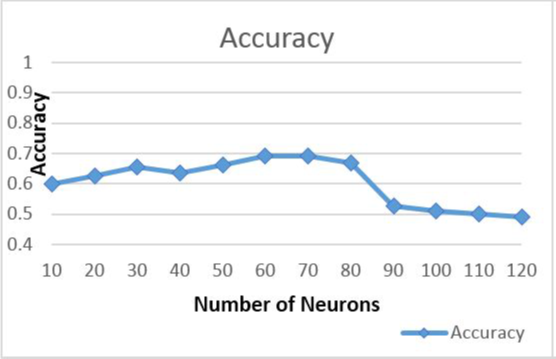
\includegraphics[width=12cm,height=6cm]{images/discuss_1.png}
    \caption{[1] Neurons vs accuracy, page 257}
    \label{fig:L1}
\end{figure} 
\begin{figure}[H]
    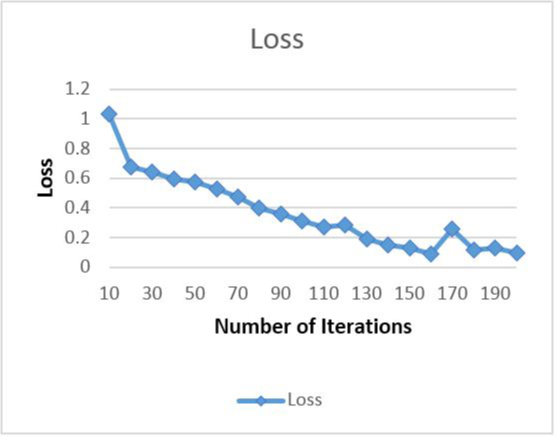
\includegraphics[width=12cm,height=6cm]{images/discuss_2.png}
    \caption{[1] Iteration vs loss, page 258}
    \label{fig:L1}
\end{figure} 
\begin{figure}[H]
    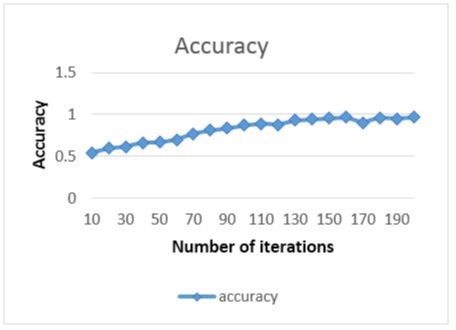
\includegraphics[width=12cm,height=6cm]{images/discuss_3.png}
    \caption{[1] Iteration vs accuracy, page 258}
    \label{fig:L1}
\end{figure} 
\begin{figure}[H]
    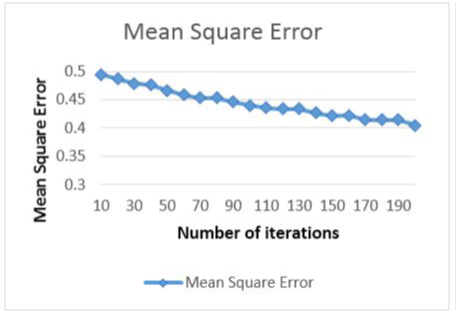
\includegraphics[width=12cm,height=6cm]{images/discuss_4.png}
    \caption{[1] Iteration vs Mean Square Error, page 258}
    \label{fig:L1}
\end{figure} 

\section{Resultats}
Avec le model du CNN sur la donnée de ISIC on obtient les resultats suivants:
$$Recall = 0.84$$
$$Precision = 0.8325$$
$$Score = 0.8325$$
d'après [2].

\newpage
\section{Conclusion}
\par Le model du CNN est un model efficace dans la détection de cellules cancéreuses. Ceci pourra aider les dermatologues dans leurs fonctions notamment à diagnostiquer plus rapidement l’enfance de la maladie du cancer. La première publication nous a permis de faire un traitement plus approfondi des images de la base de donnée, Ce qui permet au modèle de bien prédire avec plus d’efficacité.  
 


\section{Reférences}
\par [1] Mzma Bano Ansari M.E., Tanuja Sarode. Skin Cancer Detection Using Image Proceessing publié journal International Research Journal of Engineering and Technology (IRJET),\\ \url{https://www.irjet.net/archives/V4/i4/IRJET-V4I4702.pdf}\\
\par [2] Mahamudul Hasan, Samia Islam, Surajit Das Barman, Ahmed Wasif Reza. Skin Cancer Detection Using Convolutional Neural Network published in the conference: the 2019 5th International Conference in April 2019, \url{https://www.researchgate.net/publication/334751850_Skin_Cancer_Detection_Using_Convolutional_Neural_Network}


\newpage
\printbibliography
\end{document}
